% !TeX root = ../main.tex
% !TeX program = xelatex
% !TeX encoding = UTF-8
\section{负荷预测与协同优化模型}\label{minor:model}

\subsection{基本假设}

\begingroup
\setlength{\parskip}{0pt}
\newcommand{\assumptionline}[2]{\par\noindent\hangindent=1.8em\hangafter=1 #1.\hspace{0.5em}#2}
\assumptionline{1}{同类建筑参数一致时聚合为典型建筑，外部数据按 $1\,\mathrm{h}$ 步长连续输入。}
\assumptionline{2}{热源在允许工况和容量内运行，管网采用离散温位与固定温差近似，储能逐时递推且不得同时充放热。}
\par
\endgroup
\vspace{-7.5pt}

\subsection{模型结构与决策变量}

供热规划需要同时确定资产配置与逐时运行方式：热源容量决定可生产的热量，管网温位与输送能力决定热量能否到达负荷节点，储热调节供需时差，热泵、电锅炉与循环泵的用电共同占用配电容量（图\ref{fig:model-cn-overall}）。

决策变量分为三类：规划变量（热源新增与退役容量、管网保留或改造状态、储热规模、配电增容）在完整供暖季内不变；运行变量（各类热源出力、管段热流、储热充放功率、购电功率）随时段变化；状态变量（建筑热状态、储热存量）由上一时段状态与当前运行决策共同确定。规划层决定资产，运行层判断逐时可行性，校核层把不符合项转为新约束反馈重解。

\begin{figure}[H]
\centering
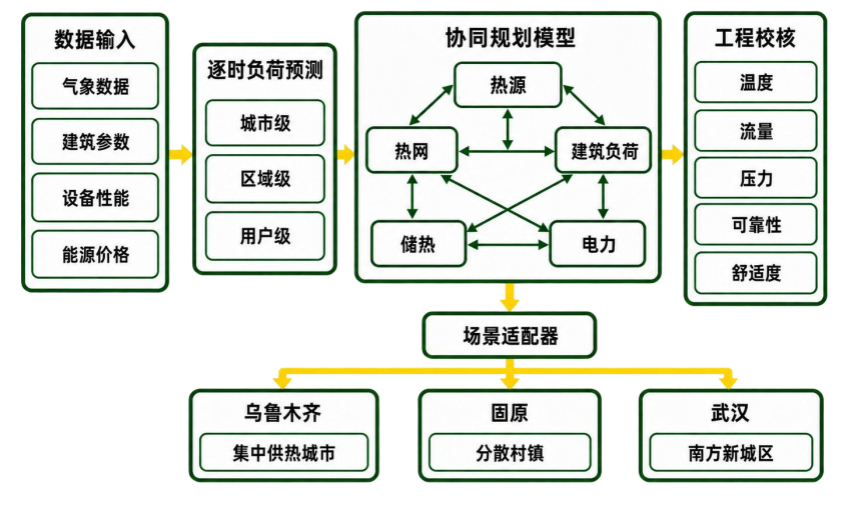
\includegraphics[width=0.62\textwidth,height=0.30\textheight,keepaspectratio]{media/model-cn/01_总体模型框架.jpg}
\caption{源网荷储电协同规划总体结构}
\label{fig:model-cn-overall}
\end{figure}

\subsection{建筑负荷与热状态}

建筑净供热负荷由围护结构传热、渗透换气与新风热损失构成，扣除太阳辐射及内部得热：

\begin{equation}
Q_{b,t}^{\mathrm{load}}
=Q_{b,t}^{\mathrm{trans}}+Q_{b,t}^{\mathrm{inf}}+Q_{b,t}^{\mathrm{vent}}
-Q_{b,t}^{\mathrm{sol}}-Q_{b,t}^{\mathrm{int}}.
\label{eq:load}
\end{equation}

其中 $U_b$、$A_b$、$n_b^{\mathrm{inf}}$、$V_b$ 为综合传热系数、围护结构面积、换气次数和建筑体积，$\theta_{b,t}^{a}$ 与 $T_t^{\mathrm{out}}$ 为室内外温度，渗透项按 $\rho_ac_an_b^{\mathrm{inf}}V_b\Delta\theta$ 逐时计算；负荷以 kW 计，参数与换算见附录\ref{app:common}。

\begin{figure}[H]
\centering
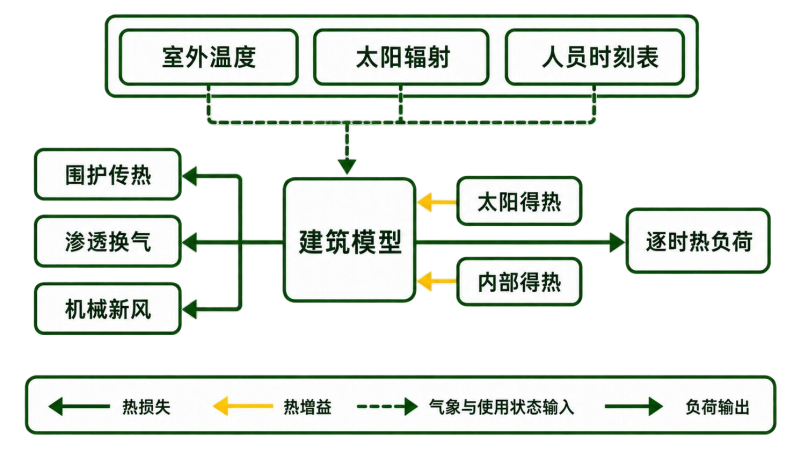
\includegraphics[width=0.58\textwidth,height=0.26\textheight,keepaspectratio]{media/model-cn/02_建筑逐时负荷分解.jpg}
\caption{建筑逐时负荷分解}
\label{fig:model-cn-load}
\end{figure}

\begin{figure}[H]
\centering
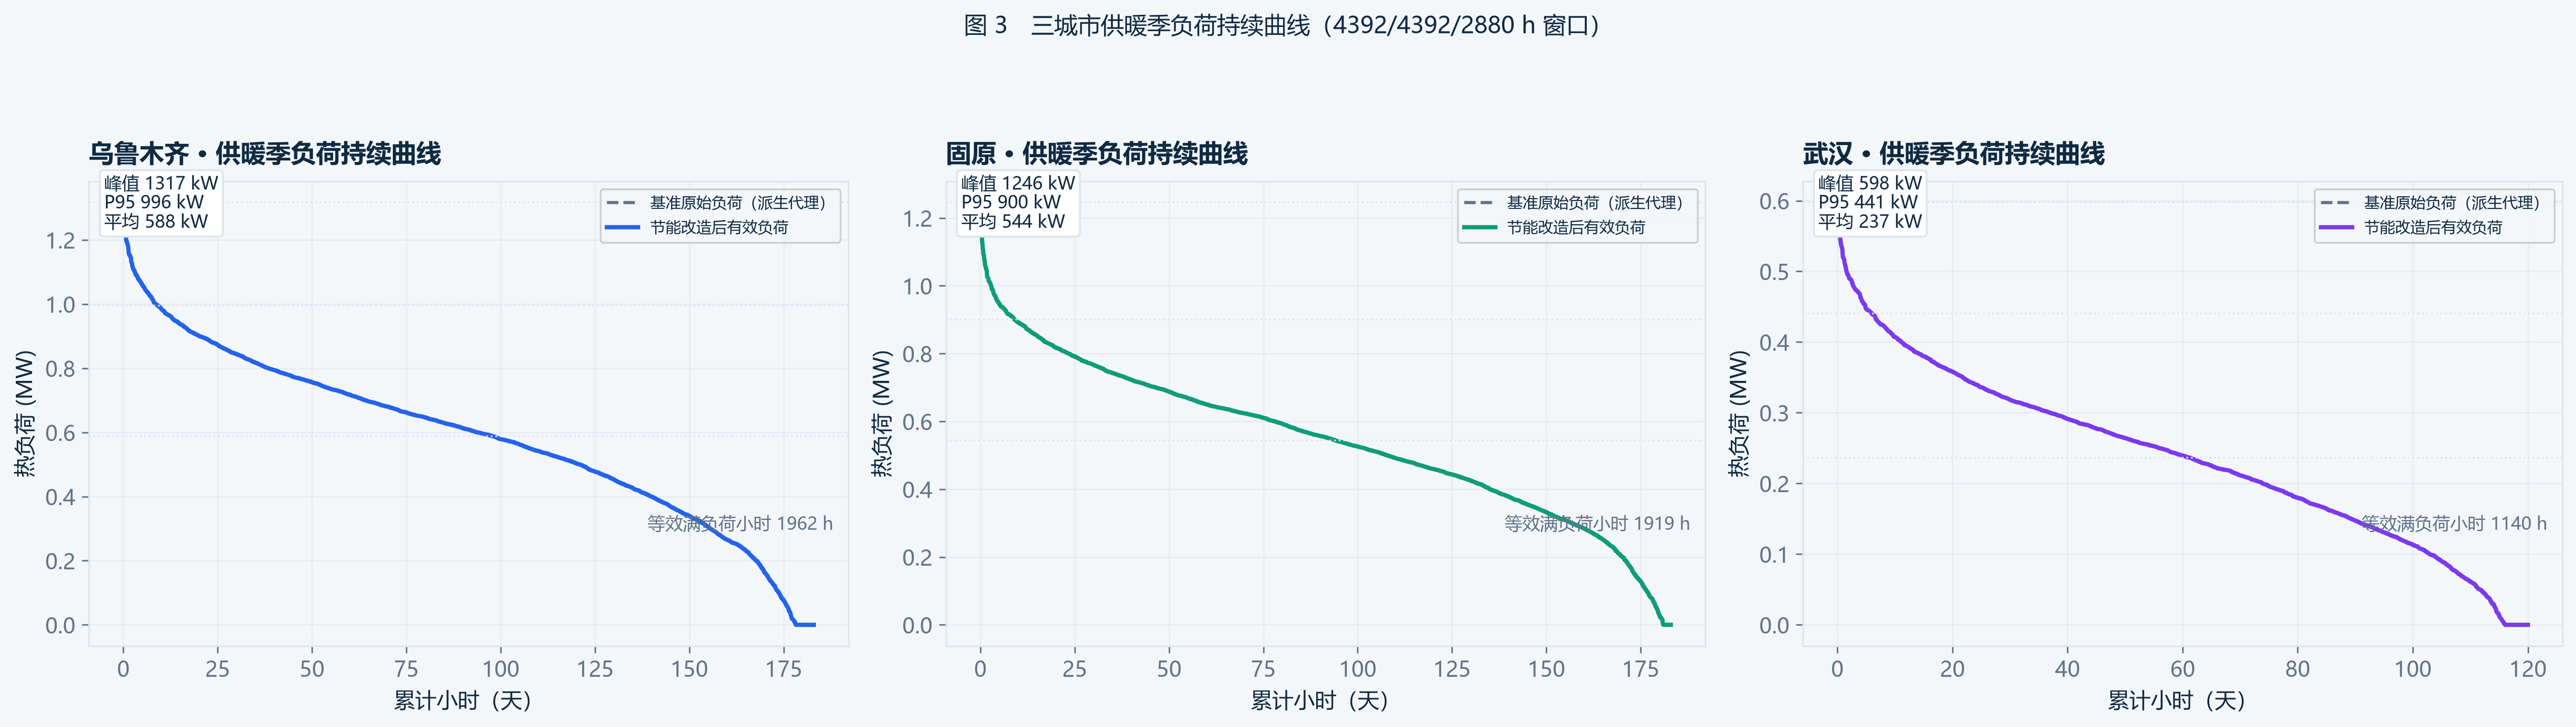
\includegraphics[width=\linewidth,height=0.22\textheight,keepaspectratio]{media/algorithm-update/fig03_load_duration_curve.png}
\caption{三城供暖季负荷持续曲线}
\label{fig:load-duration}
\end{figure}

为描述提前供热对后续室温的影响，框架列示 2R2C 结构，以室内空气温度 $\theta_{b,t}^{a}$ 与建筑质量节点温度 $\theta_{b,t}^{m}$ 为状态变量，两节点通过与外界和彼此的换热相互影响，并受舒适区间与初末状态约束：

\begin{equation}
\begin{aligned}
C_b^{a}\dfrac{\theta_{b,t+1}^{a}-\theta_{b,t}^{a}}{\Delta t}
&=Q_{b,t}^{h}-U_bA_b(\theta_{b,t}^{a}-T_t^{\mathrm{out}})
+\dfrac{\theta_{b,t}^{m}-\theta_{b,t}^{a}}{R_b^{am}}\\
&\quad-Q_{b,t}^{\mathrm{inf}}-Q_{b,t}^{\mathrm{vent}}+Q_{b,t}^{\mathrm{int}}+Q_{b,t}^{\mathrm{sol}},\\[1mm]
C_b^{m}\dfrac{\theta_{b,t+1}^{m}-\theta_{b,t}^{m}}{\Delta t}
&=\dfrac{\theta_{b,t}^{a}-\theta_{b,t}^{m}}{R_b^{am}},\\[1mm]
\theta_{b,t}^{\min}&\leq\theta_{b,t}^{a}\leq\theta_{b,t}^{\max},
\qquad
\theta_{b,1}^{a}=\theta_b^{a,0},
\qquad
\theta_{b,T}^{a}\geq\theta_b^{a,\mathrm{end}}.
\end{aligned}
\label{eq:2r2c}
\end{equation}

其中 $Q_{b,t}^{h}$ 为建筑实际获得的供热功率，$C_b^{a}$、$C_b^{m}$、$R_b^{am}$ 为空气节点热容、质量节点热容与节点间等效热阻。两式相加时节点间换热量正负相消，建筑整体只与室外和得热交换，模型封闭。下标按小时边界编号，$t=0,\dots,T$ 与首末编号同处一个窗口：给定 $\theta_b^{a,0}$ 后递推 $T$ 步，末态 $\theta_{b,T}^{a}$ 不低于登记下限。

主三城主算例使用上述结构的聚合等效形式，把建筑整体折算为单一等效热状态 $E_{n,t}$：

\begin{equation}
E_{n,t}=(1-\lambda_n)E_{n,t-1}+(q_{n,t}^{+}-q_{n,t}^{-})\Delta t,
\qquad
\Delta\theta_{n,t}=E_{n,t}/C_n.
\label{eq:agg-thermal}
\end{equation}

其中 $C_n$ 为节点 $n$ 的等效热容，$q_{n,t}^{+}$ 与 $q_{n,t}^{-}$ 为相对基准负荷的增加与削减功率，$\lambda_n$ 为逐时热损率。两式同属一个建筑热状态框架：前者保留空气与质量两个节点，说明热惯性的来源；后者是同一框架的降阶近似，以单一等效热容替代双节点网络，等效参数由登记建筑参数归并得到，误差边界不由此处的合并推出。主三城按该近似求解，逐楼精确校核由 E08 承担，见附录5。

\begin{figure}[H]
\centering
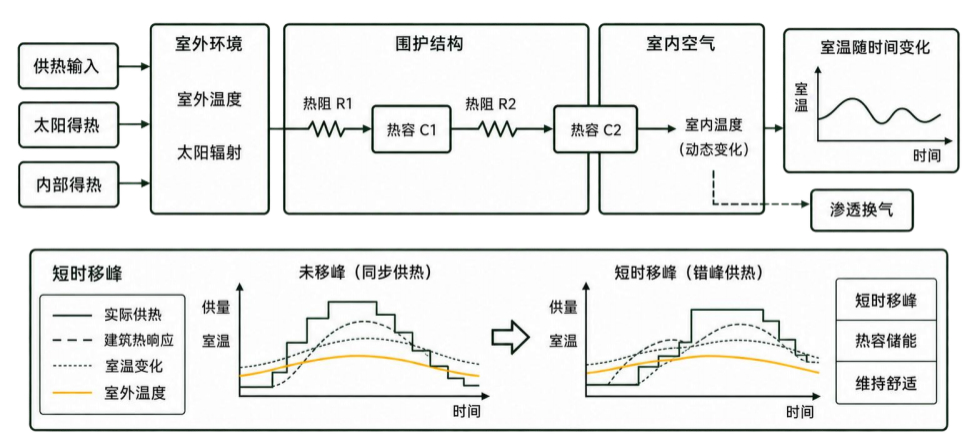
\includegraphics[width=0.58\textwidth,height=0.26\textheight,keepaspectratio]{media/model-cn/03_建筑2R2C热惯性.jpg}
\caption{建筑热惯性与跨时段移峰}
\label{fig:model-cn-2r2c}
\end{figure}

\subsection{协同约束}

\subsubsection{热源容量与能量转换}

设 $K_k^{\mathrm{exist}}$、$K_k^{\mathrm{new}}$、$K_k^{\mathrm{ret}}$ 分别为设备 $k$ 的既有、新增和退役容量，规划后容量与逐时出力满足

\begin{equation}
K_k=K_k^{\mathrm{exist}}+K_k^{\mathrm{new}}-K_k^{\mathrm{ret}},
\qquad
\underline{Q}_ku_{k,t}\leq\sum_gQ_{k,g,t}\leq a_{k,t}K_k.
\label{eq:capacity}
\end{equation}

其中 $g$ 为供热温位，$u_{k,t}$ 为启停变量，$a_{k,t}$ 为逐时可用率；设备退出运行时出力归零的完整形式，以及爬坡、最小连续运行时间与最小出力限值，见附录1.A。锅炉、热泵和电锅炉的转换关系为

\begin{equation}
Q_{k,t}^{\mathrm{boiler}}=\eta_k^{\mathrm{boiler}}F_{k,t}^{\mathrm{fuel}},
\qquad
Q_{k,t}^{\mathrm{HP}}=\mathrm{COP}_{k,t}P_{k,t}^{\mathrm{HP}},
\qquad
Q_{k,t}^{\mathrm{EB}}=\eta_k^{\mathrm{EB}}P_{k,t}^{\mathrm{EB}}.
\label{eq:conversion}
\end{equation}

直接换热与热泵源侧取同一余热时合并计入资源池，避免重复取用。

\subsubsection{节点平衡与管网输配}

按节点、温位和时段分别建立热量守恒：

\begin{equation}
\begin{aligned}
&\sum_{k\in K_n}Q_{k,g,t}
+\sum_{e\in\delta^{-}(n)}\eta_{e,t}F_{e,g,t}
+\sum_{s\in S_{n,g}}Q_{s,t}^{\mathrm{dis}}\\
&\qquad=
\sum_{b\in B_{n,g}}Q_{b,t}^{h}
+\sum_{s\in S_{n,g}}Q_{s,t}^{\mathrm{ch}}
+\sum_{e\in\delta^{+}(n)}F_{e,g,t}.
\end{aligned}
\label{eq:balance}
\end{equation}

其中 $F_{e,g,t}$ 为管段入口热功率，$\eta_{e,t}$ 为输送效率，$Q_{s,t}^{\mathrm{ch}}$ 与 $Q_{s,t}^{\mathrm{dis}}$ 为储热充、放热功率；图\ref{fig:model-cn-unified}给出各环节的热流、电力流与状态传递。

\begin{figure}[H]
\centering
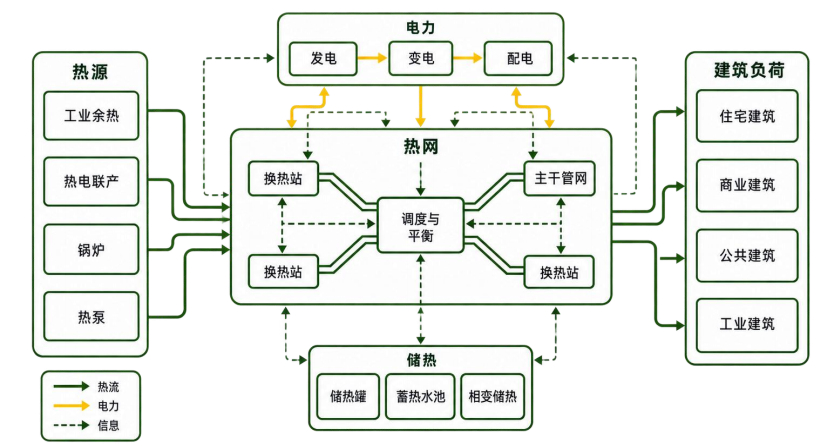
\includegraphics[width=0.60\textwidth,height=0.27\textheight,keepaspectratio]{media/model-cn/04_源网荷储电统一模型.jpg}
\caption{源网荷储电统一模型}
\label{fig:model-cn-unified}
\end{figure}

热源最低供水温度须满足

\begin{equation}
T_k^{\mathrm{src,min}}\geq T_g^{\mathrm{sup}}+\Delta T_g^{\mathrm{hx}},
\label{eq:grade}
\end{equation}

不满足式(\ref{eq:grade})的低品位热源需经热泵升温后承担高温负荷。主模型以给定供回水温差关联热功率与流量并限制管段输送容量，候选方案确定后再复算连续温降与远端压降。

\begin{figure}[H]
\centering
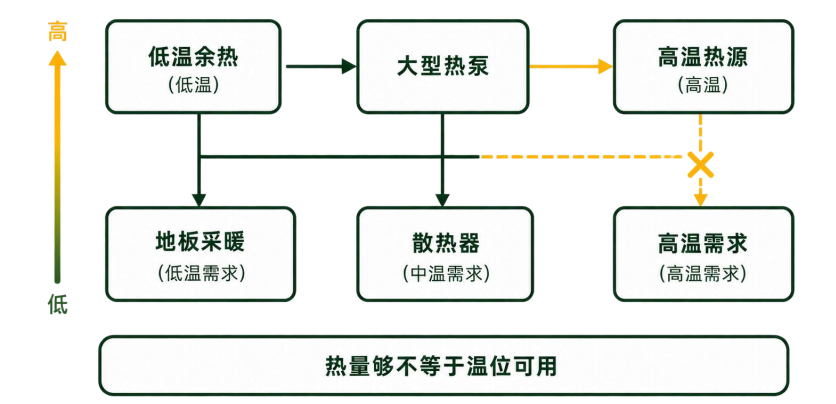
\includegraphics[width=0.58\textwidth,height=0.25\textheight,keepaspectratio]{media/model-cn/06_温位匹配与梯级利用.jpg}
\caption{温位匹配与梯级利用}
\label{fig:model-cn-grade}
\end{figure}

\subsubsection{储热与配电}

储热存量按完整供暖季连续递推，并受容量、充放功率与初末存量边界限制：

\begin{equation}
\begin{cases}
E_{s,t}=(1-\mu_s)E_{s,t-1}
+\eta_s^{\mathrm{ch}}Q_{s,t}^{\mathrm{ch}}\Delta t
-\dfrac{Q_{s,t}^{\mathrm{dis}}\Delta t}{\eta_s^{\mathrm{dis}}},\\[1mm]
0\leq E_{s,t}\leq K_s^{E},
\qquad
0\leq Q_{s,t}^{\mathrm{ch}},Q_{s,t}^{\mathrm{dis}}\leq r_sK_s^{E}.
\end{cases}
\label{eq:storage}
\end{equation}

其中 $\mu_s$ 为自损失率，$\eta_s^{\mathrm{ch}}$ 与 $\eta_s^{\mathrm{dis}}$ 为充、放热效率；模型以二元变量排除同时充放热并设置初末存量边界。热泵、电锅炉与循环泵共同占用配电容量：

\begin{equation}
(1+\sigma)
\left(
\sum_k\frac{Q_{k,t}^{\mathrm{HP}}}{\mathrm{COP}_{k,t}}
+\sum_k\frac{Q_{k,t}^{\mathrm{EB}}}{\eta_k^{\mathrm{EB}}}
+\sum_eP_{e,t}^{\mathrm{pump}}
\right)
\leq a_t^{\mathrm{grid}}K^{\mathrm{grid}}.
\label{eq:grid}
\end{equation}

该约束使热源电气化、建筑预热和储热调峰同受配电边界限制（完整形式见附录\ref{app:common}）。

\begin{figure}[H]
\centering
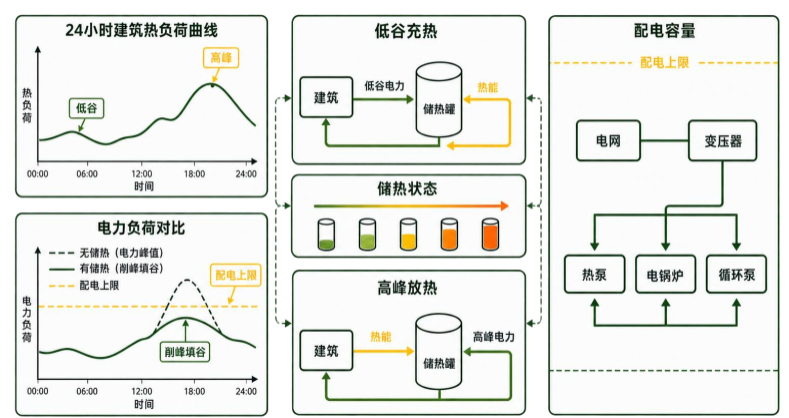
\includegraphics[width=0.60\textwidth,height=0.26\textheight,keepaspectratio]{media/model-cn/07_储热与配电协同.jpg}
\caption{储热与配电容量协同}
\label{fig:model-cn-storage-grid}
\end{figure}

\subsubsection{目标函数与可靠性}

模型以等年值成本 $F^{\mathrm{cost}}$ 最小为基础目标，并采用 $\varepsilon$ 约束控制碳排放：

\begin{equation}
\begin{cases}
\min F^{\mathrm{cost}},\\
F^{\mathrm{CO_2}}\leq\varepsilon,\\
U^{\mathrm{un}}=0.
\end{cases}
\label{eq:objective}
\end{equation}

其中等年值成本含年化投资、固定运维、燃料、购电与启停费用，碳排放按同一组燃料消耗和购电量核算，失供率为失供热量与需求热量的时间加权比。

\begin{figure}[H]
\centering
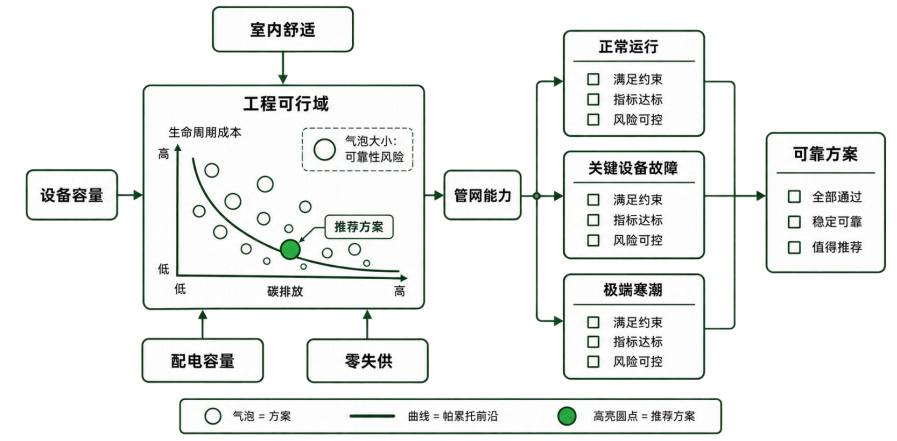
\includegraphics[width=0.58\textwidth,height=0.25\textheight,keepaspectratio]{media/model-cn/08_多目标与可靠性约束.jpg}
\caption{目标函数与可靠性约束}
\label{fig:model-cn-objective}
\end{figure}

\subsection{场景适配}

三类场景共享式(\ref{eq:load})--式(\ref{eq:objective})构成的公共内核，并按既有资产、资源条件与供能对象加载专用约束；完整约束组与极端工况见附录1.B、1.C与1.D。

\subsubsection{乌鲁木齐：既有集中供热系统低碳重构}

燃煤退役容量须由新增清洁热源、储热有效容量与备用容量共同补足：

\begin{equation}
K_{\mathrm{coal},y}^{\mathrm{ret}}
\leq K_y^{\mathrm{clean,new}}+K_y^{\mathrm{storage,credit}}+K_y^{\mathrm{reserve}}.
\label{eq:retirement}
\end{equation}

工业余热取用量受资源可得性限制，低温余热经热泵升温后承担高温负荷；任一关键热源退出时，其余热源与储热仍须覆盖逐时需求：

\begin{equation}
\begin{cases}
0\leq Q_t^{\mathrm{waste}}\leq\eta^{\mathrm{recovery}}Q_t^{\mathrm{available}},\\
Q_t^{\mathrm{HP}}=\mathrm{COP}_tP_t^{\mathrm{HP}},\\
\displaystyle\sum_{j\neq k}Q_{j,t}^{\mathrm{available}}+Q_t^{\mathrm{storage,dis}}\geq D_t.
\end{cases}
\label{eq:urumqi_key}
\end{equation}

\begin{figure}[H]
\centering
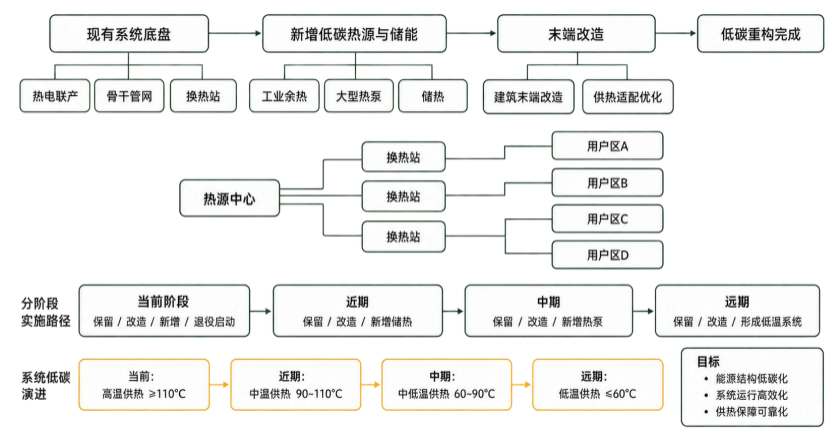
\includegraphics[width=0.58\textwidth,height=0.25\textheight,keepaspectratio]{media/model-cn/09_乌鲁木齐低碳重构.jpg}
\caption{乌鲁木齐既有集中供热低碳重构}
\label{fig:model-cn-urumqi}
\end{figure}

\subsubsection{固原与武汉：分散替代、综合供能新建}

固原每个用户仅由一个已建热源服务，并同时满足服务半径、峰值容量与生物质到货库存约束；武汉在独立楼宇、区域能源站、低温热网与第五代区域供热供冷系统间选择供能形态，选定后须逐时满足采暖和生活热水需求，低温末端表面温度不得低于露点安全温度。两类完整形式见附录1.C与1.D。

\subsection{统一校核}

模型以 $1\,\mathrm{h}$ 为分辨率完成声明窗口计算，上一时段的建筑热状态、储热量和燃料库存作为下一时段初值，不在日期边界重置。三类场景采用同一组验收条件：

\begin{equation}
\max_{n,g,t}|r_{n,g,t}^{Q}|\leq\varepsilon_Q,
\qquad
\max_{s,t}|r_{s,t}^{E}|\leq\varepsilon_E,
\label{eq:acceptance}
\end{equation}

聚合热状态处于登记区间，管段流量利用率不超 1，配电容量满足，失供率为零。代表日仅用于生成候选容量；方案确定后固定规划变量，以原始逐时序列连续回放 $T$ 小时，任一时段越界即反馈重解。
